\documentclass[11pt]{article}
\usepackage{graphicx}
\usepackage{listings}
\usepackage{color}
\usepackage[margin=1.2in]{geometry}
\usepackage{courier}
\usepackage{float}
\usepackage[toc,page]{appendix}
\usepackage{amsmath}
\usepackage{hyperref}
\usepackage{booktabs}
\usepackage{multirow}
\usepackage{setspace}
\usepackage{enumitem}

\definecolor{codegreen}{rgb}{0,0.6,0}
\definecolor{codeblack}{rgb}{0,0,0}
\definecolor{codered}{rgb}{0.867,0,0}
\definecolor{backcolour}{rgb}{ 0.95,0.95,0.95}
\definecolor{codeorange}{rgb}{1,0.447059,0}
\definecolor{codegrey}{rgb}{0.1, 0.1, 0.1}
\definecolor{codeblue}{rgb}{0.29, 0.52, 0.56}
\lstdefinestyle{mystyle}{
    basicstyle=\ttfamily\color{codeblack},
    backgroundcolor=\color{backcolour},   
    commentstyle=\color{codered},
    keywordstyle=\color{codeorange},
    numberstyle=\color{codeblack},
    stringstyle=\color{codegreen},
    breakatwhitespace=false,         
    breaklines=true,                 
    captionpos=b,                    
    keepspaces=true,                 
    numbers=left,                    
    numbersep=10pt,                  
    showspaces=false,                
    showstringspaces=false,
    showtabs=false,                  
    tabsize=3
}
 
\lstset{style=mystyle}


\twocolumn
\begin{document}
\title{CCE3015 - Programming Parallel Architectures - Assignment 1 Report}
\author{Daniel Cauchi}
\date{}
\maketitle

\section{Introduction - The Problem} \label{intro}
Fractals are figures in which a pattern occurs recursively in infinitely smaller scales. A very popular fractal is the Mandelbrot Set, which shows when a given complex number will diverge when input into the formula $f(z) = z^2 + c$. This work focuses on creating a tree fractal. The simple idea is that we start with a vertical line, then from this first line, 2 more straight lines are drawn from the upper vertex of the first line at some angle at equal distance from each other. These will be called the children lines, while the original line will be called the parent line. Then from these 2 children lines, another 2 are drawn from each line, for which the first line is the grandparent, and so on. The angles at which the new lines are drawn may vary, however in this work, an equal angle between the 2 lines is considered, where the first child line is drawn at an angle $angle_{parent} + \theta$ while the second child line is at $angle_{parent} - \theta$. Note that this is a recursive definition. The first line, as stated, is a vertical line, and this first angle will be considered as the 0 angle, so that the children will have angles at $0\pm \theta$. The length of the children are different from that to the parent, but equal to each other. A constant real number $m$ is set at the start, and the children are of length $length_{parent} * m$ (another recursive definition). An example of these concepts is in figure \ref{general explanation}, with an explanation of the terms in the next section. This report will be discussing the serial implementation of this problem while discussing the necessary preparation for the parallel implementation as well as presenting some obtained results accompanied by graphs using Matplotlib \cite{matplotlib}. Interesting to note is that other variants of this problem exists, such as parents having more than three children, or the width of the branches also changing each generation. However, this implementation will cover a binary tree fractal with constant branch width (to be distinguished from length). In the next section, the process as well as the variables of this implementation are discussed. During the research section of this project, I was not able to find any parallel implementation of this particular fractal, hence none will be discussed. \cite{natureofcode} does however provide a detailed explanation of the problem and also gives a recursive pseudo code serial implementation.

\begin{figure}
	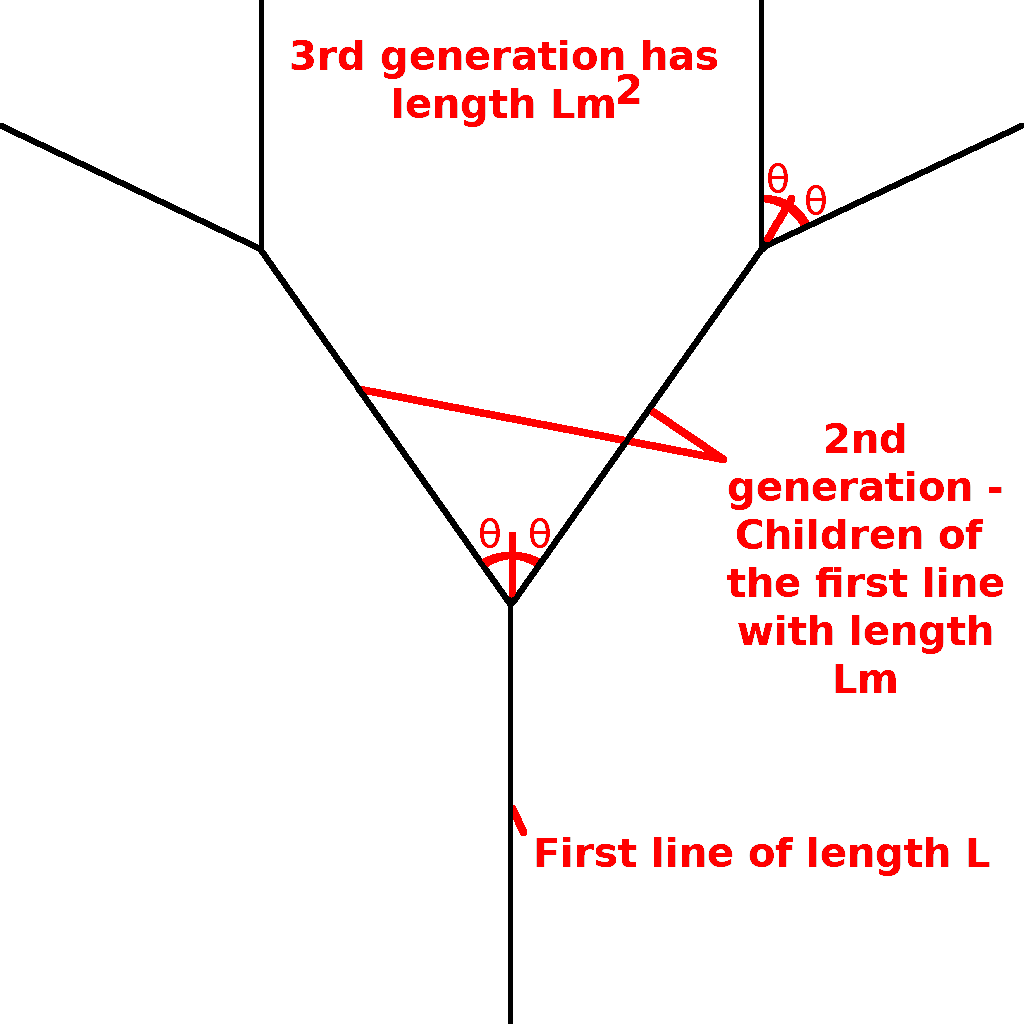
\includegraphics[width=\linewidth]{Images/GeneralExplanation.png}
	\centering
	\caption{A fractal generated by the program, with $\theta=30$, $m=0.6$ and $n=3$}
	\label{general explanation}
\end{figure}

\section{Implementation and Pipeline}
The implementation of this problem is split into several parts. First, the required user inputs are discussed:
\begin{enumerate}
	\item Image width $W$ - The width of the pgm image which will be the final artefact obtained by the program
	\item Image height $H$ - The height of the output image
	\item Length multiplier $m$ - The value by which the length of the parent will be multiplied to get the length of its children (discussed in section \ref{intro})
	\item Rotation per iteration $\theta$ - The angle with which the child lines will diverge from that of the parent (discussed in section \ref{intro})
	\item Number of iterations $n$ - How many generations of lines there will be. 1 means that only the first line is drawn.
\end{enumerate}
Next, the several stages of the pipeline to get the desired image are discussed.

First, a cosine and sine list is generated, which maps an angle to its result in sine or cosine. These were generated for angles between -180 to 180 degrees, at an interval of 1, which means the angles in degrees must be an integer. This is a limitation, albeit not a harsh one, but leads to a significant optimization so that the sine and cosine function do not need to be called for each line, since these functions are computationally demanding. Instead, to get an angle after generating the map, one can simply do: $sin\_list[\theta + 180]$ to get $sin(\theta)$, and the same with cosine. This also means that the angle $\theta$ must be between -180 and 179 (both included) otherwise the index for the array will go out of bounds.

After this list is generated, we can compute the points for the lines. The first two points for the first line are initialised as $(0, 0)$ and $(0, 1)$. Note how the length of the first line will always be taken as 1. This is because when synthesizing the image, the generated tree will be made to stretch to the image size, hence this initial length will not matter. This design choice was taken because it will not allow any space in the image to be wasted and more importantly so that the tree will not go out of the image bounds. To get the next 2 lines, the principle of matrix multiplication is used (hence the need of the sine and cosine maps). So the 2 new points are first placed at $(0, length_{parent} * m)$, then a rotation of $\pm parent_{angle} + \theta$ is applied and finally the position of the parent is added to these points to get their new positions. The 2 new lines will later be drawn from the end of the parent to the 2 new generated points. A list of the angles of each line also needs to be kept as the children's angle depends on the parents'.

The final step before synthesising the image (drawing the lines), is to map the points from coordinate space to image/pixel space. This is needed due to image space starting at $(0, 0)$ at its top-left corner, while coordinate space has $(0,0)$ at the bottom middle. Therefore, in order to perform this conversion, the following operations are performed: 
\\ \\
$x_{image} = \\ x_{coordinate} * W / (x_{min} - x_{max}) + image_width/2$
\\ \\
$y_{image} = y_{coordinate} * - H / (y_{max} - y_{min}) + H - H*(y_{max}-y_{min}) * y_{min}$
\\ \\\
where $x_{max}$ and $x_{min}$ are the maximum and maximum X values in coordinate space accordingly, and the same for the Y values. Furthermore, as stated before, W is the image width and H is the image height. Note that $x_{min}$ is $-x_{max}$ since the tree is symmetric across x. Also important to state is that only the variables with subscript \textit{coordinate} are variables, while the others are constant, which leads to options for optimizations, such that the computation for each point becomes
\\ \\
$x_{image} = x_{coordinate} * x_{mul} + x_{add}$
\\ \\
and similarly for y. This will be very useful when it comes to parallelization.

The final step of the pipeline is synthesizing the image. This is done by moving one pixel at a time in some axis from one point towards the other point. However, say we have only the first line to render, and we move in the x-axis. If this is done, then we end up with just 1 pixel drawn. Therefore, the approach taken is to move in the axis for which the distance between the points in that axis is biggest. So for a mostly horizontal line, we move in the x-axis, and if we have a mostly vertical line, we move pixel by pixel in the y-axis. To determine how much is needed to be moved in the other axis, this is calculated initially. To explain this better, an example is given: Say that we have 2 points, one of them at $(0, 0)$ and the other at $(2, 7)$. The first thing to notice is that the biggest difference is in the y-axis. Therefore we will move pixel by pixel from point 0 to point 7 in the y-axis. To find the corresponding x values, we find how much we need to move at each step. The formula for this is $(x_{max}-x_{min})/y_{difference} = (2-0)/7 = 0.286$, so we start at $x=0$ when $y=0$, and when y moves by 1, x moves by 0.286, then the resulting float is rounded to an integer to find the pixel position to draw. With this way, this difference is only calculated once per line. At y=7, x will be equal to 2.

Therefore, in short, this is the pipeline:
\begin{enumerate}
	\item Populate the sin and cosine maps
	\item Generate the points
	\item Transform the points from coordinate space to image space
	\item Draw the points to synthesize the image
\end{enumerate}


With regards to a data structure for the points, while a binary tree may be used and may be more elegant, a simpler structure is used, that of 2 arrays. The first array stores the results of the x-values while the second stores the y-values. The parent points of a child are found using the following formula: $x_{parent} = floor(x_{child}/2)$, and similarly for y. So the children of the point at index 1 has children at indexes 2 and 3, then point 2 has children at indexes 4 and 5 while 3 has children at indexes 6 and 7. Point 0 is the special starting point at $(0, 0)$. The advantage to this is that iteration may be used for calculating the points rather than recursion, and when parallelizing, it is easier to copy an array rather than a binary tree. This same structure is used for the angles for each line.
\section{Choice of problem and Options for Parallelization}
While this problem is not fully parallelizable, different parts of the pipeline are parallelizable. This problem was chosen for this reason, because it will be interesting to investigate if parallelization will make this problem faster. Each part of the pipeline will now be taken into consideration, discussing its time and space complexity and its amenability to parallelization:

\begin{enumerate}
	\item Populating the sine and cosine maps: An O(1) operation, performing a total of 360 sin operations and 360 cos operations. Populating each map is parallelizable, where each thread performs a single sine or cosine operation
	\item Generating the points and angles for each line: An O($2^n$) operation, where n is the number of iterations. Here both the x and y coordinates need to be generated, however each iteration depends on the last one to finish first. An optimisation can be done to compute the first $<block dimension>$ points in one kernel call with a $syncthreads()$ call within a for loop. For the other iterations, however, the device will need to finish all operations, then be synchronised by the host before starting the next iteration. Note: After generating the points, the memory for the angles may be freed.
	\item Mapping the coordinate space points to image space is fully parallelizable, as this consists of one multiplication and one addition per axis per point. This operation is also O($2^n$) since the number of points has this complexity
	\item The last part of the pipeline is the image synthesis. Here, each thread may compute a line. It will not matter if both threads write the the same pixel at a time, because the operation is changing a pixel from white to black, hence if one overwrites the other in a random order, the result is still the same. The complexity of this operation is not so straight forward as it depends on the image size, hence this will be determined graphically in section \ref{results}.
\end{enumerate}

Another part which may be parallellized in the case of this implementation is the initialisation of the image matrix, to make it all white at the start.

An important thing to note is that before a step in the pipeline starts, the last step of the pipeline must finish.

With regards to memory, the only thing which will be needed to be copied to the host memory is the image matrix, while everything else may be initialised and remain in memory until it is freed. In terms of memory complexity, this is O($2^n$), as it mostly depends on the number of points to be determined. In exact bytes, we have $2^n * (sizeof(short) * sizeof(float) * 2)$ where the shorts are the list of angles for each point and the floats are the coordinates, one for x and one for y. Then there is also the addition of the sine and cosine maps as well as the image matrix, however these are negligible compared to the size of the other items which depend on the number of iterations. For the points however, a limit of 26 iterations is set, because at 26 iterations, $2^n$ will need 640 MB of memory, as the size of a short is typically 2 bytes while the size of a float is typically 4 bytes, meaning the bytes are $10*2^n$.
\section{Testing and Results} \label{results}


\section{Conclusion}
This concludes this report for the serial implementation of creating tree fractals. A description of how this solution can be implemented serially was discussed. A general idea on how this solution may be parallellized is presented and finally results were shown using graphs to display how long the pipeline of the problem takes. A study on the time complexity of the problem was also made for completion.

\bibliography{main}
\bibliographystyle{ieeetr}

\pagebreak

%\input{Subfiles/Appendix}

\end{document}